\documentclass[class=minimal,border=10pt]{standalone}
\usepackage{lmodern}
\usepackage{tikz}
\usepackage{xcolor}
\definecolor{blue}{RGB}{65,105,225}
\definecolor{cyan}{RGB}{42,161,152}
\definecolor{base01}{RGB}{88,110,117}
\definecolor{base02}{RGB}{50, 50, 50}
\definecolor{base03}{RGB}{0,43,54}
\usetikzlibrary{calc,shapes,positioning}
\begin{document}
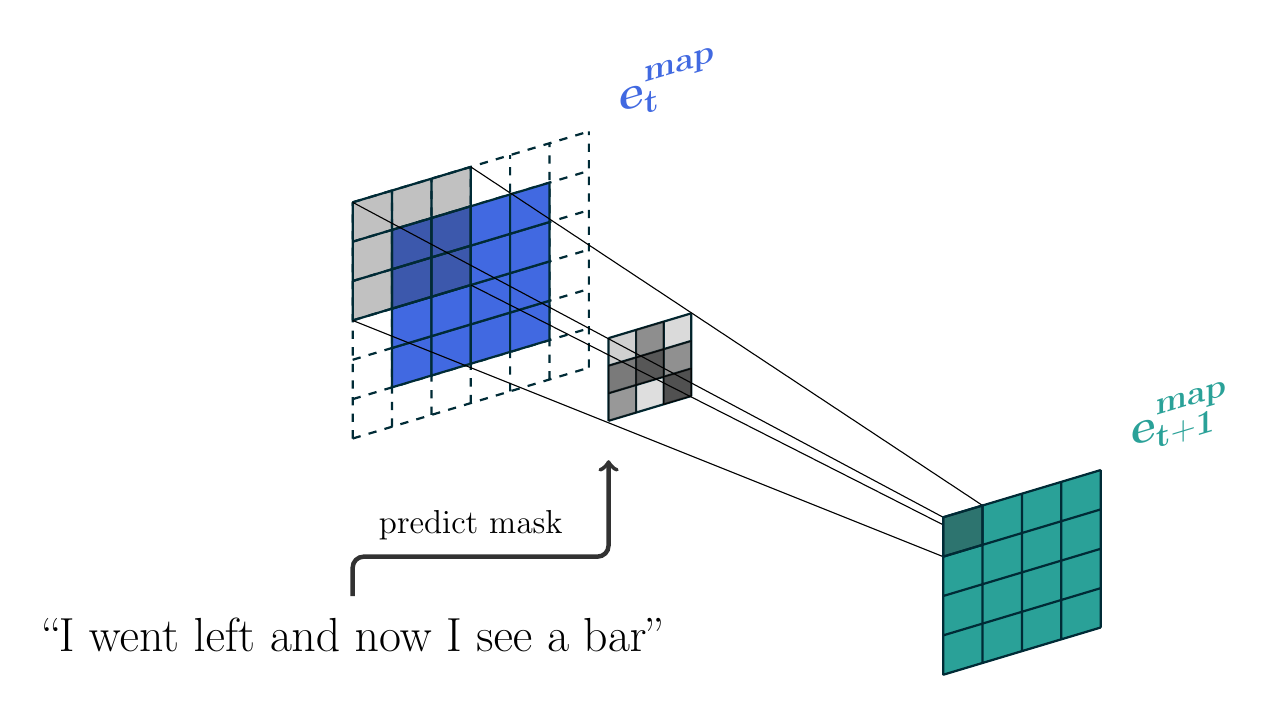
\begin{tikzpicture}[scale=.5,every node/.style={minimum size=1cm},on grid]
    \begin{scope}[node/.append style={yslant=0.3,xslant=0.0},
                    yslant=0.3,xslant=0.0]
        \draw[step=10mm, base03, dashed, thick] (0,0) grid (6,6);
        \draw[draw=base03, fill=blue, thick] (1,1) rectangle (2,2);
        \draw[draw=base03, fill=blue, thick] (1,2) rectangle (2,3);
        \draw[draw=base03, fill=blue, thick] (1,3) rectangle (2,4);
        \draw[draw=base03, fill=blue, thick] (1,4) rectangle (2,5);
        \draw[draw=base03, fill=blue, thick] (2,1) rectangle (3,2);
        \draw[draw=base03, fill=blue, thick] (2,2) rectangle (3,3);
        \draw[draw=base03, fill=blue, thick] (2,3) rectangle (3,4);
        \draw[draw=base03, fill=blue, thick] (2,4) rectangle (3,5);
        \draw[draw=base03, fill=blue, thick] (3,1) rectangle (4,2);
        \draw[draw=base03, fill=blue, thick] (3,2) rectangle (4,3);
        \draw[draw=base03, fill=blue, thick] (3,3) rectangle (4,4);
        \draw[draw=base03, fill=blue, thick] (3,4) rectangle (4,5);
        \draw[draw=base03, fill=blue, thick] (4,1) rectangle (5,2);
        \draw[draw=base03, fill=blue, thick] (4,2) rectangle (5,3);
        \draw[draw=base03, fill=blue, thick] (4,3) rectangle (5,4);
        \draw[draw=base03, fill=blue, thick] (4,4) rectangle (5,5);


        \draw[fill=base02, opacity=0.3] (0, 3) rectangle (1,4);
        \draw[fill=base02, opacity=0.3] (1, 3) rectangle (2,4);
        \draw[fill=base02, opacity=0.3] (2, 3) rectangle (3,4);
        \draw[fill=base02, opacity=0.3] (0, 4) rectangle (1,5);
        \draw[fill=base02, opacity=0.3] (1, 4) rectangle (2,5);
        \draw[fill=base02, opacity=0.3] (2, 4) rectangle (3,5);
        \draw[fill=base02, opacity=0.3] (0, 5) rectangle (1,6);
        \draw[fill=base02, opacity=0.3] (1, 5) rectangle (2,6);
        \draw[fill=base02, opacity=0.3] (2, 5) rectangle (3,6);
        \draw[step=10mm, base03, thick] (0, 3) grid
                                        (3, 6);
        \coordinate (BL) at (0,3);
        \coordinate (BR) at (3,3);
        \coordinate (TL) at (0,6);
        \coordinate (TR) at (3,6);

    \end{scope}

    \begin{scope}[xshift=6.5cm, yshift=0.45cm,
                    every node/.append style={yslant=0.3,xslant=0.0},
                    yslant=0.3,xslant=0.0]
        \draw[step=7mm, base03, thick] (0, 0) grid
                                        (2.1, 2.1);

        \draw[fill=base02, opacity=0.5] (0, 0) rectangle (0.7,0.7);
        \draw[fill=base02, opacity=0.16] (0.7, 0) rectangle (1.4, 0.7);
        \draw[fill=base02, opacity=0.85] (1.4, 0) rectangle (2.1, 0.7);
        \draw[fill=base02, opacity=0.65] (0, 0.7) rectangle (0.7,1.4);
        \draw[fill=base02, opacity=0.82] (0.7, 0.7) rectangle (1.4, 1.4);
        \draw[fill=base02, opacity=0.54] (1.4, 0.7) rectangle (2.1, 1.4);
        \draw[fill=base02, opacity=0.23] (0, 1.4) rectangle (0.7,2.1);
        \draw[fill=base02, opacity=0.55] (0.7, 1.4) rectangle (1.4, 2.1);
        \draw[fill=base02, opacity=0.18] (1.4, 1.4) rectangle (2.1, 2.1);
        \coordinate (IC) at (0, -1.0);
    \end{scope}
    \begin{scope}[xshift=15cm, yshift=-6cm,
                    every node/.append style={yslant=0.3,xslant=0.0},
                    yslant=0.3,xslant=0.0]
        \draw (BL) -- (0,3) (BR) -- (1,3)
              (TL) -- (0,4)    (TR) -- (1,4);
        \draw[fill=cyan] (0,0) rectangle (4,4);
        \draw[step=10mm, base03, thick] (0,0) grid (4,4);
        \draw[fill=base02, opacity=0.4] (0,3) rectangle
                                        (1,4);
        \draw[base03, thick] (0,3) rectangle (1,4);
    \end{scope}
    \begin{scope}[xshift=0cm, yshift=-5cm]
        \node[font=\fontsize{16}{0}\selectfont] {``I went left and now I see a bar''};
        \draw[->, rounded corners, color=base02, ultra thick]  (0, 1)  -- (0, 2) -- (6.5, 2) -- (IC);
    \end{scope}
    \begin{scope}[xshift=3cm, yshift=-2.2cm]
        \node[font=\fontsize{12}{0}\selectfont] {predict mask};
    \end{scope}
    \begin{scope}[xshift=8cm,yshift=9cm, every node/.append style={yslant=0.3,xslant=0.0}]
        \node[rectangle, color=blue, font=\fontsize{18}{0}\selectfont] {$\mathbf{e^{map}_t}$};
    \end{scope}
    \begin{scope}[xshift=21cm,yshift=0.5cm, every node/.append style={yslant=0.3,xslant=0.0}]
        \node[rectangle, color=cyan, font=\fontsize{18}{0}\selectfont] {$\mathbf{e^{map}_{t+1}}$};
    \end{scope}
\end{tikzpicture}
\end{document}